%%%%%%%%%%%%%%%%%%%%%%
% Chapter mini-intro %
%%%%%%%%%%%%%%%%%%%%%%



%%%%%%%%%%%%%%%%%%%%%%%%%%
% Parlato1 (Interspeech) %
%%%%%%%%%%%%%%%%%%%%%%%%%%

%%%% Main %%%%
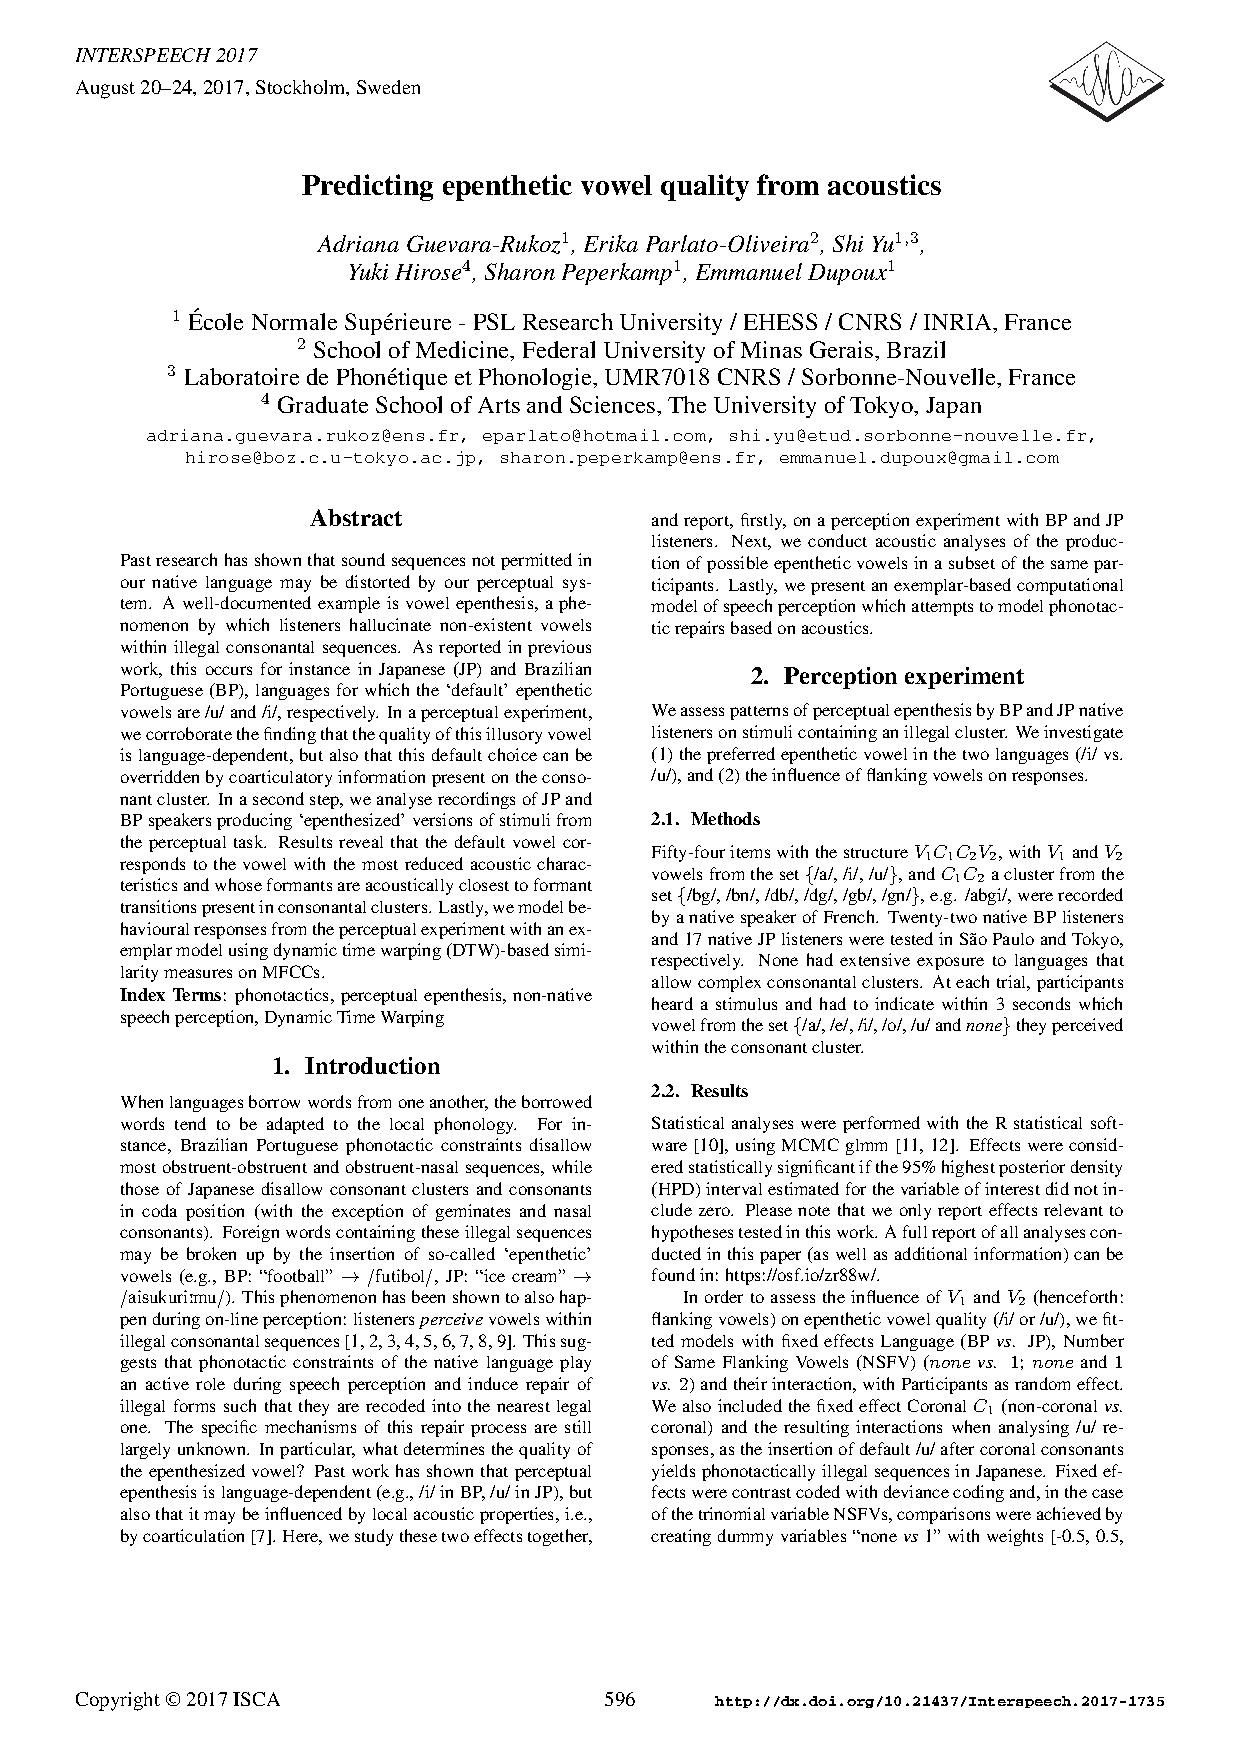
\includepdf[pages={1-5},pagecommand={},
addtotoc={
  1,section,1,Predicting epenthetic vowel quality from acoustics,parlato1_main,
  1,subsection,2,Perception experiment,parlato1_per,
  2,subsection,2,Acoustic analyses,parlato1_prod,
  3,subsection,2,Production-based exemplar model,parlato1_mod,
  4,subsection,2,Discussion,parlato1_disc,
  5,subsection,2,References,parlato1_ref
}]
{images/chapter02/Interspeech2017_Predicting_epenthetic_vowel_quality_from_acoustics_final.pdf}

%%%% Annexes %%%%
\subsection{Annexes}

\subsubsection{Human and model responses at identification task} 

\subsubsection{/i/-epenthesis} 
\begin{figure}[H]
  \centering
  \begin{overpic}[page=1, width=0.4\linewidth]{chapter02/parlato_per_iou}\end{overpic}
  \hspace{1cm}
  \begin{overpic}[page=3, width=0.4\linewidth]{chapter02/parlato_per_iou}\end{overpic}
  \caption{Proportion of /i/-epenthesis in the perception experiment with BP and JP participants (left) and the simulations with the corresponding exemplar-based models (right). Bigger dots show mean values, while smaller dots show individual values for human participants.}
  \label{fig:parlato_uepenth}
\end{figure}

\subsubsection{/u/-epenthesis} 
\begin{figure}[H]
  \centering
  \begin{overpic}[page=2, width=0.4\linewidth]{chapter02/parlato_per_iou}\end{overpic}
  \hspace{1cm}
  \begin{overpic}[page=4, width=0.4\linewidth]{chapter02/parlato_per_iou}\end{overpic}
  \caption{Proportion of /u/-epenthesis in the perception experiment with BP and JP participants (left) and the simulations with the corresponding exemplar-based models (right). Bigger dots show mean values, while smaller dots show individual values for human participants.}
  \label{fig:parlato_uepenth}
\end{figure}

\subsubsection{Acoustic analyses} 
\begin{figure}[H]
  \centering
  \begin{overpic}[clip, trim=0 0 0 0, page=1, height=6.5cm]{chapter02/parlato_acoustic}\end{overpic}
  \hspace{0.5cm}
  \begin{overpic}[clip, trim=0 0 0 0, page=2, height=6.5cm]{chapter02/parlato_acoustic}\end{overpic}
  \begin{overpic}[clip, trim=0 0 0 0, page=3, height=6.5cm]{chapter02/parlato_acoustic}\end{overpic}
  \caption{Acoustic properties of medial vowels /i, o, u/ produced by BP and JP participants. Distribution of log'd vowel duration (in ms), median intensity (in dB) and square root Euclidean distance to template in F1 x F2 x F3 space (frequencies in Bark). Dashed lines show mean values.}
  \label{fig:parlato_prod}
\end{figure}

%\newpage

%%%%%%%%%%%%%%%%%%%%
% /ahpa/ (JASA-EL) %
%%%%%%%%%%%%%%%%%%%%

%%%% Main %%%%
\includepdf[pages={2-8}, pagecommand={},
addtotoc={
  2,section,1,Which epenthetic vowel? \\ Phonetic categories versus acoustic detail in perceptual vowel epenthesis,ahpa_main,
  3,subsection,2,Methods,ahpa_methods,
  4,subsection,2,Results,ahpa_results,
  6,subsection,2,Discussion,ahpa_disc,
  7,subsection,2,References,ahpa_ref}]
{images/chapter02/JASAEL_Guevara-Rukoz_2017_Which_epenthetic_vowel.pdf}

%%%% Annexes %%%%
\subsection{Annexes}

\subsubsection{Acoustic analyses}
%[TODO] Add graphs 

\subsubsection{ABX task}

% [TODO] Copied from rebuttal letter; edit
% [TODO] Add correlation results + graph
We also performed a control ABX task with a different set of participants, as this task promotes a more global perception of the stimuli. In this experiment, participants heard trials with 4 types of AB pairs:
\begin{itemize}
    \item $V_1CpV_1$ (non-spliced cluster) vs. $V_1CV_1pV_1$ (full vowel)
    \item $V_1CpV_1$ (non-spliced cluster) vs. $V_1C_{V_2}pV_1$ (spliced cluster)
    \item $V_1C_{V_2}pV_1$ (spliced cluster) vs. $V_1C_{V_3}pV_1$ (spliced cluster)
    \item $V_1C_{V_2}pV_1$ (spliced cluster) vs. $V_1CV_2pV_1$ (full vowel)
\end{itemize}

We saw that ABX accuracy rates for each pair were correlated with how similar response patterns for items A and B were at the identification task. In other words, the more similar response patterns were for A and B at the identification task, the harder it was for participants to discriminate A and B at the ABX task. \\

Similarity of responses was assessed by computing the Euclidean distance between 6-dimensional vectors [$p_{none}$, $p_a$, $p_e$, $p_i$, $p_o$, $p_u$] of A and B, where $p_x$ corresponds to the proportion of total trials for A (or B) in which participants responded $x$. This suggests that adaptation patterns attested in the identification task are not task-dependent.
\\

%While we did not include these results for publication because we were not entirely satisfied with the choice of pairs used (a better setup might have been to have $V_1C(_{V_2})pV_1$ vs. $V_1CV_{1/2}pV_1$ pairs, in order to tackle our questions more directly), results of this ABX experiment, as well as their correlation to results from the identification task described in the manuscript, are available in https://osf.io/y9h6c/, which we update continuously based on questions that may arise during this revision process, during presentations, when colleagues contact us in relation to the project, etc. 

%%%%%%%%%%%%%%%%%%%%%%%%%%%
% Chapter mini-discussion %
%%%%%%%%%%%%%%%%%%%%%%%%%%%